\scanpage{155}
{\ttfamily
* \unsure{LE NIVEAU DU SYSTEME} MVS/SP \unsure{1.3|1.1} SERA MIS EN SERVICE SUR LE *\\
* 3081 LE 21 AOUT 1982. *\\
*\hfill *\\
******************************************************************}
\figure{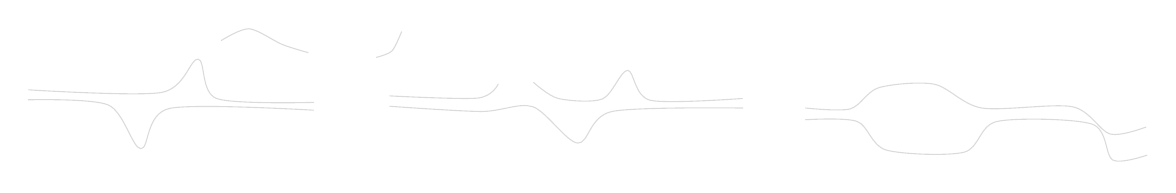
\begin{tikzpicture}[x=.55cm,y=-.55cm,line cap=round,line join=round,g/.style={olive!80!yellow,line width=1.7pt},r/.style={orange!80!brown,line width=1.8pt},w/.style={red!60!black,line width=1.5pt},b/.style={blue!60!black,line width=1.4pt},p/.style={gray!70,thin},k/.style={black,line width=1.2pt},every node/.style={font=\scriptsize}]
\draw[p,opacity=.4] plot[smooth] coordinates {(1.8,2.97) (4.87,3.03) (5.71,2.26) (6.14,3.17) (8.38,3.26)};
\draw[p,opacity=.4] plot[smooth] coordinates {(1.79,3.2) (3.64,3.32) (4.39,4.33) (5.05,3.4) (8.38,3.44)};
\draw[p,opacity=.4] plot[smooth] coordinates {(6.25,1.83) (6.89,1.56) (7.65,1.92) (8.25,2.11)};
\draw[p,opacity=.4] plot[smooth] coordinates {(9.83,2.22) (10.19,2.07) (10.41,1.63)};
\draw[p,opacity=.4] plot[smooth] coordinates {(10.14,3.11) (12.17,3.16) (12.64,2.84)};
\draw[p,opacity=.4] plot[smooth] coordinates {(10.14,3.35) (12.25,3.47) (13.44,3.36) (14.48,4.2) (15.27,3.47) (18.29,3.39)};
\draw[p,opacity=.4] plot[smooth] coordinates {(13.46,2.8) (14.03,3.17) (15.05,3.18) (15.63,2.52) (16.15,3.21) (18.28,3.17)};
\draw[p,opacity=.4] plot[smooth] coordinates {(19.74,3.39) (20.77,3.41) (21.43,2.92) (22.71,2.84) (23.81,3.39) (25.9,3.36) (26.77,3.99) (27.6,3.83)};
\draw[p,opacity=.4] plot[smooth] coordinates {(19.74,3.66) (20.93,3.7) (21.6,4.36) (23.4,4.41) (24.16,3.7) (26.35,3.76) (26.83,4.59) (27.62,4.48)};
\end{tikzpicture}}
balayages élémentaires de positions relatives
\figure{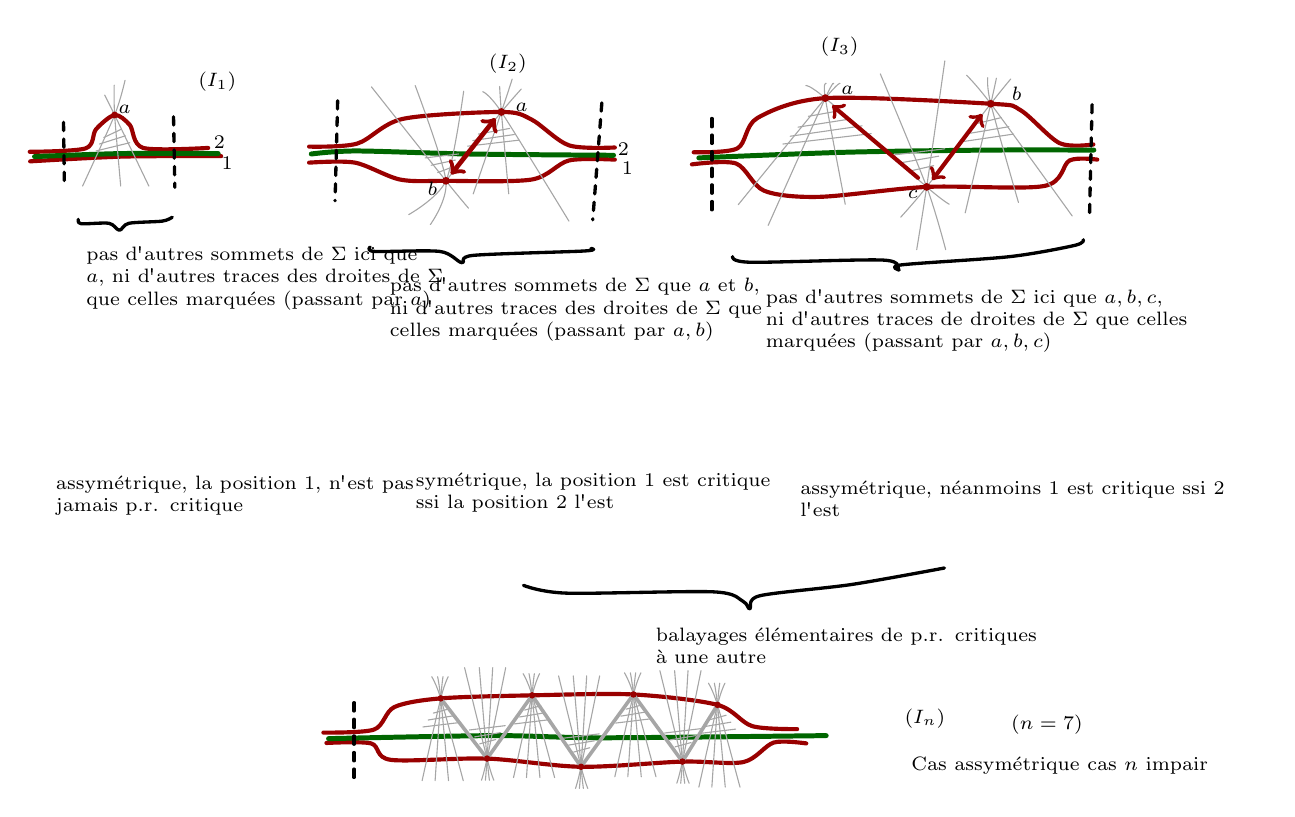
\begin{tikzpicture}[x=.55cm,y=-.55cm,line cap=round,line join=round,g/.style={olive!80!yellow,line width=1.7pt},r/.style={orange!80!brown,line width=1.8pt},w/.style={red!60!black,line width=1.5pt},b/.style={blue!60!black,line width=1.4pt},p/.style={gray!70,thin},k/.style={black,line width=1.2pt},every node/.style={font=\scriptsize}]
\draw[w] plot[smooth] coordinates {(2.87,7.0) (4.16,6.92) (4.4,6.48) (4.83,6.15) (5.18,6.38) (5.49,6.91) (6.99,6.91)};
\draw[w] plot[smooth] coordinates {(2.88,7.22) (5.02,7.11) (7.29,7.1)};
\draw[green!40!black,line width=1.8pt] plot[smooth] coordinates {(2.98,7.11) (5.0,7.04) (7.22,7.04)};
\draw[p] plot[smooth] coordinates {(4.6,5.69) (4.83,6.15) (5.62,7.79)};
\draw[p] plot[smooth] coordinates {(5.07,5.35) (4.83,6.15) (4.09,7.79)};
\draw[p] plot[smooth] coordinates {(4.82,5.46) (4.83,6.15) (4.97,7.79)};
\draw[p] plot[smooth] coordinates {(4.58,6.67) (4.98,6.48)};
\draw[p] plot[smooth] coordinates {(4.48,6.82) (5.08,6.63)};
\draw[p] plot[smooth] coordinates {(4.4,6.98) (5.18,6.79)};
\draw[k,dashed] plot[smooth] coordinates {(3.65,6.32) (3.67,7.75)};
\draw[k,dashed] plot[smooth] coordinates {(6.19,6.19) (6.22,7.82)};
\fill[w] (4.83,6.15) circle (.08);
\node at (5.06,6.03) {$a$};
\node at (7.2,5.39) {$(I_1)$};
\node at (7.25,6.79) {$2$};
\node at (7.43,7.26) {$1$};
\draw[k] plot[smooth] coordinates {(3.99,8.56) (4.06,8.66) (4.7,8.65) (4.94,8.81) (5.16,8.65) (5.93,8.6) (6.16,8.51)};
\node[anchor=north west,align=left,text width=4.7cm] at (3.95,8.98) {pas d\textquotesingle autres sommets de $\Sigma$ ici que $a$, ni d\textquotesingle autres traces des droites de $\Sigma$ que \deleted{\unsure{celles}} marquées (passant par $a$)};
\node[anchor=north west,align=left,text width=4.7cm] at (3.25,14.25) {\uline{assymétrique}, la position 1, n\textquotesingle est \uline{pas} \deleted{\unsure{jamais}} p.r. critique};
\draw[w] plot[smooth] coordinates {(9.32,6.88) (10.43,6.81) (11.48,6.24) (13.76,6.08) (14.45,6.25) (15.32,6.85) (16.38,6.9)};
\draw[w] plot[smooth] coordinates {(9.32,7.25) (10.38,7.25) (11.42,7.64) (12.48,7.67) (14.46,7.64) (15.32,7.2) (16.38,7.18)};
\draw[green!40!black,line width=1.8pt] plot[smooth] coordinates {(9.37,7.05) (10.4,6.98) (13.0,7.05) (16.35,7.08)};
\draw[p] plot[smooth] coordinates {(10.76,5.5) (12.48,7.67) (13.0,8.3)};
\draw[p] plot[smooth] coordinates {(11.77,5.47) (12.48,7.67) (12.12,8.68)};
\draw[p] plot[smooth] coordinates {(12.89,5.6) (12.48,7.67) (11.62,8.45)};
\draw[p] plot[smooth] coordinates {(13.11,7.97) (13.76,6.08) (14.01,5.32)};
\draw[p] plot[smooth] coordinates {(13.33,5.61) (13.76,6.08) (15.32,8.6)};
\draw[p] plot[smooth] coordinates {(13.72,5.49) (13.76,6.08) (13.93,7.97)};
\draw[p] plot[smooth] coordinates {(14.22,5.55) (13.76,6.08) (12.48,7.67)};
\draw[p] plot[smooth] coordinates {(12.98,6.87) (14.17,6.73)};
\draw[p] plot[smooth] coordinates {(13.1,6.74) (14.06,6.6)};
\draw[p] plot[smooth] coordinates {(13.23,6.59) (13.95,6.46)};
\draw[p] plot[smooth] coordinates {(12.0,7.14) (12.77,7.05)};
\draw[p] plot[smooth] coordinates {(12.14,7.31) (12.7,7.19)};
\draw[p] plot[smooth] coordinates {(12.29,7.48) (12.58,7.37)};
\draw[w,<->,line width=1.7pt] plot[smooth] coordinates {(12.6,7.52) (13.62,6.23)};
\draw[k,dashed] plot[smooth] coordinates {(9.98,5.82) (9.92,8.13)};
\draw[k,dashed] plot[smooth] coordinates {(16.08,5.87) (15.87,8.57)};
\fill[w] (13.76,6.08) circle (.09);
\fill[w] (12.48,7.67) circle (.09);
\node at (14.23,5.98) {$a$};
\node at (12.17,7.86) {$b$};
\node at (13.91,4.96) {$(I_2)$};
\node at (16.58,6.94) {$2$};
\node at (16.67,7.39) {$1$};
\draw[k] plot[smooth] coordinates {(10.73,9.2) (10.84,9.3) (12.34,9.3) (12.85,9.56) (13.12,9.39) (15.67,9.29) (15.83,9.23)};
\node[anchor=north west,align=left,text width=4.8cm] at (10.96,9.7) {pas d\textquotesingle autres sommets de $\Sigma$ que $a$ et $b$, ni d\textquotesingle autres traces des droites de $\Sigma$ que celles marquées (passant par $a,b$)};
\node[anchor=north west,align=left,text width=4.8cm] at (11.56,14.2) {\uline{symétrique}, la position 1 est critique ssi la position 2 l\textquotesingle est};
\draw[w] plot[smooth] coordinates {(18.2,7.01) (19.21,6.92) (19.67,6.22) (21.24,5.76) (25.06,5.89) (25.75,6.04) (26.65,6.8) (27.43,6.83)};
\draw[w] plot[smooth] coordinates {(18.16,7.29) (19.18,7.27) (19.83,7.9) (21.1,8.04) (23.58,7.81) (26.29,7.79) (26.88,7.2) (27.52,7.18)};
\draw[green!40!black,line width=1.8pt] plot[smooth] coordinates {(18.32,7.14) (21.7,7.01) (25.0,6.96) (27.44,6.96)};
\draw[p] plot[smooth] coordinates {(20.79,5.47) (21.24,5.76) (23.58,7.81) (24.1,8.21)};
\draw[p] plot[smooth] coordinates {(21.58,5.42) (21.24,5.76) (19.23,8.22)};
\draw[p] plot[smooth] coordinates {(21.26,5.42) (21.24,5.76) (21.7,8.21)};
\draw[p] plot[smooth] coordinates {(21.43,5.43) (21.24,5.76) (19.92,8.7)};
\draw[p] plot[smooth] coordinates {(22.51,5.2) (23.58,7.81) (24.02,9.26)};
\draw[p] plot[smooth] coordinates {(24.0,4.9) (23.58,7.81) (23.35,9.26)};
\draw[p] plot[smooth] coordinates {(24.5,5.23) (25.06,5.89) (26.94,8.48)};
\draw[p] plot[smooth] coordinates {(25.19,5.3) (25.06,5.89) (24.47,8.41)};
\draw[p] plot[smooth] coordinates {(25.52,5.32) (25.06,5.89) (23.58,7.81) (22.98,8.51)};
\draw[p] plot[smooth] coordinates {(24.99,5.29) (25.06,5.89) (25.7,8.17)};
\draw[p] plot[smooth] coordinates {(20.26,6.82) (22.3,6.58)};
\draw[p] plot[smooth] coordinates {(20.43,6.64) (22.09,6.4)};
\draw[p] plot[smooth] coordinates {(20.61,6.43) (21.83,6.24)};
\draw[p] plot[smooth] coordinates {(20.85,6.18) (21.57,6.05)};
\draw[p] plot[smooth] coordinates {(22.84,7.07) (24.0,6.93)};
\draw[p] plot[smooth] coordinates {(23.0,7.25) (23.86,7.1)};
\draw[p] plot[smooth] coordinates {(23.21,7.44) (23.74,7.32)};
\draw[p] plot[smooth] coordinates {(24.44,6.76) (25.59,6.59)};
\draw[p] plot[smooth] coordinates {(24.59,6.57) (25.48,6.42)};
\draw[p] plot[smooth] coordinates {(24.77,6.34) (25.3,6.21)};
\draw[w,->] plot[smooth] coordinates {(23.38,7.6) (21.4,5.93)};
\draw[w,<->] plot[smooth] coordinates {(23.71,7.65) (24.86,6.13)};
\draw[k,dashed] plot[smooth] coordinates {(18.62,6.23) (18.62,8.43)};
\draw[k,dashed] plot[smooth] coordinates {(27.4,5.91) (27.34,8.5)};
\fill[w] (21.24,5.76) circle (.09);
\fill[w] (25.06,5.89) circle (.09);
\fill[w] (23.58,7.81) circle (.09);
\node at (21.75,5.58) {$a$};
\node at (25.66,5.66) {$b$};
\node at (23.26,7.98) {$c$};
\node at (21.57,4.57) {$(I_3)$};
\draw[k] plot[smooth] coordinates {(19.1,9.42) (19.52,9.55) (22.58,9.5) (22.94,9.73) (23.0,9.61) (25.5,9.42) (27.0,9.16) (27.2,9.03)};
\node[anchor=north west,align=left,text width=5.9cm] at (19.64,9.97) {pas d\textquotesingle autres sommets de $\Sigma$ ici que $a,b,c$, ni d\textquotesingle autres traces de droites de $\Sigma$ que celles marquées (passant par $a,b,c$)};
\node[anchor=north west,align=left,text width=5.8cm] at (20.44,14.37) {\uline{assymétrique}, néanmoins 1 est critique ssi 2 l\textquotesingle est};
\draw[k] plot[smooth] coordinates {(14.27,17.01) (15.26,17.19) (18.65,17.16) (19.34,17.38) (19.5,17.55) (19.73,17.25) (21.85,16.99) (23.99,16.61)};
\node[anchor=north west,align=left,text width=5cm] at (17.1,17.76) {balayages élémentaires de p.r. critiques \unsure{à une} \unsure{autre}};
\draw[w] plot[smooth] coordinates {(9.65,20.41) (10.82,20.34) (11.29,19.82) (12.36,19.62) (14.47,19.55) (16.81,19.53) (18.75,19.77) (19.55,20.26) (20.59,20.33)};
\draw[w] plot[smooth] coordinates {(9.72,20.65) (10.75,20.66) (11.21,21.04) (13.43,21.01) (15.6,21.2) (17.94,21.08) (19.35,21.09) (20.05,20.64) (20.8,20.66)};
\draw[green!40!black,line width=1.8pt] plot[smooth] coordinates {(9.77,20.55) (13.59,20.48) (16.1,20.53) (21.26,20.48)};
\draw[k,dashed] plot[smooth] coordinates {(10.36,19.72) (10.36,21.55)};
\draw[p,line width=1.3pt] (12.36,19.62)--(13.43,21.01)--(14.47,19.55)--(15.6,21.2)--(16.81,19.53)--(17.94,21.08)--(18.75,19.77);
\draw[p] plot[smooth] coordinates {(12.532,19.12) (12.36,19.62) (11.93,21.52)};
\draw[p] plot[smooth] coordinates {(12.411999999999999,19.12) (12.36,19.62) (12.229999999999999,21.52)};
\draw[p] plot[smooth] coordinates {(12.288,19.12) (12.36,19.62) (12.54,21.52)};
\draw[p] plot[smooth] coordinates {(12.152,19.12) (12.36,19.62) (12.879999999999999,21.52)};
\draw[p] (12.19,19.96)--(12.559999999999999,19.86);
\draw[p] (12.07,20.12)--(12.669999999999998,20.02);
\draw[p] (11.95,20.28)--(12.78,20.18);
\draw[p] plot[smooth] coordinates {(13.86,18.91) (13.43,21.01) (13.301,21.51)};
\draw[p] plot[smooth] coordinates {(13.56,18.91) (13.43,21.01) (13.391,21.51)};
\draw[p] plot[smooth] coordinates {(13.25,18.91) (13.43,21.01) (13.484,21.51)};
\draw[p] plot[smooth] coordinates {(12.91,18.91) (13.43,21.01) (13.586,21.51)};
\draw[p] (13.26,20.67)--(13.629999999999999,20.57);
\draw[p] (13.14,20.51)--(13.739999999999998,20.41);
\draw[p] (13.02,20.35)--(13.85,20.25);
\draw[p] plot[smooth] coordinates {(14.642000000000001,19.05) (14.47,19.55) (14.040000000000001,21.45)};
\draw[p] plot[smooth] coordinates {(14.522,19.05) (14.47,19.55) (14.34,21.45)};
\draw[p] plot[smooth] coordinates {(14.398000000000001,19.05) (14.47,19.55) (14.65,21.45)};
\draw[p] plot[smooth] coordinates {(14.262,19.05) (14.47,19.55) (14.99,21.45)};
\draw[p] (14.3,19.89)--(14.67,19.79);
\draw[p] (14.180000000000001,20.05)--(14.78,19.95);
\draw[p] (14.06,20.21)--(14.89,20.11);
\draw[p] plot[smooth] coordinates {(16.03,19.099999999999998) (15.6,21.2) (15.471,21.7)};
\draw[p] plot[smooth] coordinates {(15.73,19.099999999999998) (15.6,21.2) (15.561,21.7)};
\draw[p] plot[smooth] coordinates {(15.42,19.099999999999998) (15.6,21.2) (15.654,21.7)};
\draw[p] plot[smooth] coordinates {(15.08,19.099999999999998) (15.6,21.2) (15.756,21.7)};
\draw[p] (15.43,20.86)--(15.799999999999999,20.759999999999998);
\draw[p] (15.31,20.7)--(15.909999999999998,20.599999999999998);
\draw[p] (15.19,20.54)--(16.02,20.439999999999998);
\draw[p] plot[smooth] coordinates {(16.982,19.03) (16.81,19.53) (16.38,21.43)};
\draw[p] plot[smooth] coordinates {(16.862,19.03) (16.81,19.53) (16.68,21.43)};
\draw[p] plot[smooth] coordinates {(16.738,19.03) (16.81,19.53) (16.99,21.43)};
\draw[p] plot[smooth] coordinates {(16.602,19.03) (16.81,19.53) (17.33,21.43)};
\draw[p] (16.639999999999997,19.87)--(17.009999999999998,19.77);
\draw[p] (16.519999999999996,20.03)--(17.119999999999997,19.93);
\draw[p] (16.4,20.19)--(17.229999999999997,20.09);
\draw[p] plot[smooth] coordinates {(18.37,18.979999999999997) (17.94,21.08) (17.811,21.58)};
\draw[p] plot[smooth] coordinates {(18.07,18.979999999999997) (17.94,21.08) (17.901,21.58)};
\draw[p] plot[smooth] coordinates {(17.76,18.979999999999997) (17.94,21.08) (17.994,21.58)};
\draw[p] plot[smooth] coordinates {(17.42,18.979999999999997) (17.94,21.08) (18.096,21.58)};
\draw[p] (17.77,20.74)--(18.14,20.639999999999997);
\draw[p] (17.65,20.58)--(18.25,20.479999999999997);
\draw[p] (17.53,20.419999999999998)--(18.36,20.319999999999997);
\draw[p] plot[smooth] coordinates {(18.922,19.27) (18.75,19.77) (18.32,21.669999999999998)};
\draw[p] plot[smooth] coordinates {(18.802,19.27) (18.75,19.77) (18.62,21.669999999999998)};
\draw[p] plot[smooth] coordinates {(18.678,19.27) (18.75,19.77) (18.93,21.669999999999998)};
\draw[p] plot[smooth] coordinates {(18.542,19.27) (18.75,19.77) (19.27,21.669999999999998)};
\draw[p] (18.58,20.11)--(18.95,20.009999999999998);
\draw[p] (18.459999999999997,20.27)--(19.06,20.169999999999998);
\draw[p] (18.34,20.43)--(19.169999999999998,20.33);
\fill[w] (12.36,19.62) circle (.075);
\fill[w] (13.43,21.01) circle (.075);
\fill[w] (14.47,19.55) circle (.075);
\fill[w] (15.6,21.2) circle (.075);
\fill[w] (16.81,19.53) circle (.075);
\fill[w] (17.94,21.08) circle (.075);
\fill[w] (18.75,19.77) circle (.075);
\node at (23.54,20.08) {$(I_n)$};
\node at (26.36,20.23) {$(n=7)$};
\node[anchor=west] at (23.0,21.18) {Cas \unsure{assymétrique} cas $n$ impair};
\end{tikzpicture}}
\margin{\mspage{154}}
